\documentclass[a4paper, 12pt]{article}
% packages
\usepackage{amssymb}
\usepackage[fleqn]{mathtools}
\usepackage{tikz}
\usepackage{enumerate}
\usepackage{bussproofs}
\usepackage{xcolor}
\usepackage[margin=1.3cm]{geometry}
\usepackage{logicproof}
\usepackage{diagbox}
\usepackage{karnaugh-map}

% augmented matrix
\makeatletter
\renewcommand*\env@matrix[1][*\c@MaxMatrixCols c]{%
\hskip -\arraycolsep
\let\@ifnextchar\new@ifnextchar
\array{#1}}
\makeatother

% ceiling / floor
\DeclarePairedDelimiter{\ceil}{\lceil}{\rceil}
\DeclarePairedDelimiter{\floor}{\lfloor}{\rfloor}

% custom commands
\newcommand{\indefint}[2]{\int #1 \, \mathrm{d}#2}
\newcommand{\defint}[4]{\int_#1^#2 #3 \, \mathrm{d}#4}
\newcommand{\dif}[2]{\frac{\mathrm{d}#1}{\mathrm{d}#2}}
\newcommand{\limit}[2]{\displaystyle{\lim_{#1 \to #2}}}
\newcommand{\summation}[3]{\sum\limits_{#1}^#2 #3}
\newcommand{\intbracket}[3]{\left[#3\right]_#1^#2}

\newcommand{\powerset}[0]{\wp}
\renewcommand{\emptyset}[0]{\varnothing}

\newcommand{\unaryproof}[2]{\AxiomC{#1} \UnaryInfC{#2} \DisplayProof}
\newcommand{\binaryproof}[3]{\AxiomC{#1} \AxiomC{#2} \BinaryInfC{#3} \DisplayProof}

% no indent
\setlength\parindent{0pt}

% reasoning proofs
\newcommand{\proofline}[3]{(#1)\ & #2 & \text{#3} \\}
\allowdisplaybreaks

% actual document
\begin{document}
    \section*{CO112 - Hardware}
        \subsection*{Prelude}
            The content discussed here is part of CO112 - Hardware (Computing MEng); taught by Bernhard Kainz, and Bjoern Schuller, in Imperial College London during the academic year 2018/19. The notes are written for my personal use, and have no guarantee of being correct (although I hope it is, for my own sake). This should be used in conjunction with the notes, and lecture slides. This course starts off fairly slow, especially if you have an idea of how logic gates work, and therefore the first parts won't be covered in much detail.
        \subsection*{Lecture 1}
            \subsubsection*{Notes}
                This section will be covered in less detail, as we've gone through the majority of this in much greater depth during logic. However, we will need to change the notation we use in this course from the one used in logic, from using $\land$ to $\cdot$, $\lor$ to $+$, and from $\neg$ to $^\prime$.
                \begin{center}
                    \begin{tabular}{cc|c|c|c}
                        $A$ & $B$ & $A \cdot B$ (AND) & $A + B$ (OR) & $A^\prime$ (NOT) \\
                        \hline
                        0 & 0 & 0 & 0 & 1 \\
                        0 & 1 & 0 & 1 & 1 \\
                        1 & 0 & 0 & 1 & 0 \\
                        1 & 1 & 1 & 1 & 0
                    \end{tabular}
                \end{center}
                The same distributivity laws apply, just like in \textbf{CO140}, as well as the simplification laws. In general, the laws should be the same as propositional logic, with the notation being slightly changed. Use 1 for $\top$, and 0 for $\bot$. We will also be using de Morgan's theorem on any number of variables (this can be proven by induction), such that $(V_1 + V_2 + V3 + ... + V_n)^\prime \equiv V_1^\prime \cdot V_2^\prime \cdot V_3^\prime \cdot ... \cdot V_n^\prime$, and the same the other way around. This can be very useful later on, as we will often use NAND / NOR gates to reduce silicon area.
        \subsection*{Lecture 2}
            \subsubsection*{Notes}
                The three operators covered in the first lecture can be represented by three logic gates; AND, OR, and NOT. The inverter (NOT), is represented by the circle at the end of the triangle. We can also create operations such as NAND, and NOR. Any of the first three gates can be built with just NAND gates, or just NOR gates. Let us represent $A$ NAND $B$, with $A \uparrow B$.
                \begin{itemize}
                    \itemsep0em
                    \item $A^\prime$ \hfill $A \uparrow A$
                    \item $A \cdot B$ \hfill $(A \uparrow B)^\prime$
                        \subitem \hfill $(A \uparrow B) \uparrow (A \uparrow B)$
                    \item $A + B$ \hfill $(A ^\prime \cdot B^\prime)^\prime$ (de Morgan's)
                        \subitem \hfill $A^\prime \uparrow B^\prime$
                        \subitem \hfill $(A \uparrow A) \uparrow (B \uparrow B)$
                \end{itemize}
                We also need to introduce two new gates, which are commonly used in digital logic; XOR, and XNOR. Roughly, you can use the same rules for $\neg (A \leftrightarrow B)$, and $A \leftrightarrow B$ respectively. XOR is commonly represented by $A \oplus B$ (which is much shorter than $A \cdot B^\prime + A^\prime \cdot B$), and XNOR represented by $(A \oplus B)^\prime$, instead of $A^\prime \cdot B^\prime + A \cdot B$. It has the following truth table;
                \begin{center}
                    \begin{tabular}{cc|c|c}
                        $A$ & $B$ & $A \oplus B$ & $(A \oplus B)^\prime$ \\
                        \hline
                        0 & 0 & 0 & 1 \\
                        0 & 1 & 1 & 0 \\
                        1 & 0 & 1 & 0 \\
                        1 & 1 & 0 & 1
                    \end{tabular}
                \end{center}
                In general, with $n$ inputs, we can have $2^n$ unique gates.
                With this information, we can build a single control block. For example, let there be a block with an input $A$, a control $C$, and output $R$. It follows that if $C$ is 0, then the output is 0, and $A$, if $C$ is 1. Hence $R = A \cdot C$.
                \medskip

                Now, if we had something with two inputs, $A$, and $B$, and a control $C$, we could use $C$ to determine whether $R = A$, or $R = B$. This is done with the boolean equation $R = A \cdot C^\prime + B \cdot C$. This is a \textbf{multiplexer}, which will be used very often in circuit design for other components.
        \subsection*{Lecture 3}
            \subsubsection*{Notes}
                Consider an more complex circuit, where we have 3 outputs; $R_1, R_2$, and $R_3$, and 4 inputs; $A, B, C$, and $D$, where $R_n=f_n(A, B, C, D)$. For now, we ignore sequential circuits, where the output can be on either side of the equation. The first step of creating a circuit is to construct a truth table as a starting point. We also need to define a few terms;
                \begin{itemize}
                    \itemsep0em
                    \item \textbf{minterm} - a boolean product where each input, or its complement, appears exactly once
                        \subitem hence $A \cdot B^\prime \cdot C$ is a minterm, but $A \cdot B$ isn't.
                        \subitem also known as sum-of-products, or disjunction-of-conjunctions
                    \item \textbf{maxterm} - a boolean sum where each input, or its complement, appears exactly once
                        \subitem hence $A + B^\prime + C$ is a minterm, but $A + B$ isn't.
                        \subitem also known as product-of-sums, or conjunction-of-disjunctions
                \end{itemize}
                For example, let's work on the following truth table;
                \begin{center}
                    \begin{tabular}{c|c|c|c|c}
                        $A$ & $B$ & $C$ & $R$ & \\
                        \hline
                        0 & 0 & 0 & 0 & maxterm $A + B + C$ \\
                        0 & 0 & 1 & 0 & maxterm $A + B + C^\prime$ \\
                        0 & 1 & 0 & 0 & maxterm $A + B^\prime + C$ \\
                        0 & 1 & 1 & 1 & minterm $A \cdot B \cdot C$ \\
                        1 & 0 & 0 & 0 & maxterm $A^\prime + B + C$ \\
                        1 & 0 & 1 & 1 & minterm $A \cdot B^\prime \cdot C$ \\
                        1 & 1 & 0 & 1 & minterm $A \cdot B \cdot C^\prime$ \\
                        1 & 1 & 1 & 1 & minterm $A \cdot B \cdot C$
                    \end{tabular}
                \end{center}
                Now, we can evaluate $R$ in two ways;
                \begin{itemize}
                    \itemsep0em
                    \item $R = (A \cdot B \cdot C) + (A \cdot B^\prime \cdot C) + (A \cdot B \cdot C^\prime) + (A \cdot B \cdot C)$ \hfill sum of minterms
                    \item $R = (A + B + C) \cdot (A + B + C^\prime) \cdot (A + B^\prime + C) \cdot (A^\prime + B + C)$ \hfill product of maxterms
                \end{itemize}
                Knowing this, we can convert any truth table into a \textbf{Karnaugh map}
                \begin{center}
                    \begin{tabular}{c|c|c|c|c||c|c|c|c|c}
                        $A$ & $B$ & $C$ & $D$ & $R$ & $A$ & $B$ & $C$ & $D$ & $R$ \\
                        \hline
                        0 & 0 & 0 & 0 & 0 & 1 & 0 & 0 & 0 & 1 \\
                        0 & 0 & 0 & 1 & 1 & 1 & 0 & 0 & 1 & 1 \\
                        0 & 0 & 1 & 0 & 1 & 1 & 0 & 1 & 0 & 1 \\
                        0 & 0 & 1 & 1 & 1 & 1 & 0 & 1 & 1 & 1 \\
                        0 & 1 & 0 & 0 & 0 & 1 & 1 & 0 & 0 & 1 \\
                        0 & 1 & 0 & 1 & 1 & 1 & 1 & 0 & 1 & 1 \\
                        0 & 1 & 1 & 0 & 1 & 1 & 1 & 1 & 0 & 1 \\
                        0 & 1 & 1 & 1 & 0 & 1 & 1 & 1 & 1 & 1
                    \end{tabular}

                    \begin{karnaugh-map}[4][4][1][$CD$][$R:\ AB$]
                        \manualterms{0, 1, 1, 1, 0, 1, 1, 0, 1, 1, 1, 1, 1, 1, 1, 1}
                        \implicant{12}{10}
                        \implicant{1}{9}
                        \implicant{3}{2}
                        \implicant{6}{6}
                    \end{karnaugh-map}
                \end{center}
                Hence we can use minterms, to get $R = \underbrace{A}_\text{red} + \underbrace{C^\prime \cdot D}_\text{green} + \underbrace{A^\prime \cdot B^\prime \cdot C}_\text{yellow} + \underbrace{A^\prime \cdot B \cdot C \cdot D^\prime}_\text{blue}$. 
                \medskip

                Remember that the regions in the map can wrap around, and that don't cares can count as either 0, or 1.
        \subsection*{Lecture 4}
            \subsubsection*{Notes}
                A general circuit can be used to generate all possible $n$-input digital circuits. If we were to have inputs $V_1, V_2, ..., V_n$, and have each one come out as two lines, so $V_i$ would come out with $V_i$, and its complement $V_i^\prime$. We can have $2^n$ $n$-input AND gates, which correspond to each possible combination (00...00), (00...01), (00...11), all the way to (11...11). This is hard to visualise (see \textit{Notes04 - Description to Circuit.pdf}), but the general idea is that each AND gate corresponds to a possible minterm, which is joined to a $2^n$-input OR gate, if it's a 1 in the truth table. This is a \textbf{Programmable Array Logic (PAL)} device, and the device can be prgrammed by sending a current through specific links to connect them to the OR gate.
                \medskip

                The general steps for creating a device from a specified device are as follows;
                \begin{enumerate}[1.]
                    \itemsep0em
                    \item Construct a truth table
                        \subitem translate the natural language description of what the device should do into a truth table.
                    \item Generate a Karnaugh map
                        \subitem using the techniques mentioned in the previous lecture, create the map, and find the resulting sum of minterms (or product of maxterms)
                    \item Minimise the boolean expression
                        \subitem using the resulting sum or product, we can then use boolean algebra to simplify the expression
                    \item Design the circuit
                        \subitem using the minimised boolean expression, we can finally construct a circuit
                    \item Minimise the circuit
                        \subitem this is different from minimising the equation, as we're now trying to minimise the silicon area used
                        \subitem in general, this is to replace ANDs, and ORs, with NANDs, and NORs
                        \subitem a method of doing this is to replace expressions such as $(A \cdot B)$ with $(A^\prime + B^\prime)^\prime$, by using de Morgan's law
                    \item Test the circuit
                        \subitem the usual process is to simulate the circuit, to validate it against the original specifications
                        \subitem finding bugs before production is important (and expensive, if not spotted); see the \textit{Floating Point Division Bug} in \textit{Intel Pentium P5}
                \end{enumerate}
        \subsection*{Lecture 5}
            \subsubsection*{Pantopo}
                While boolean algebra is a good abstraction for the behaviour of logic gates, it has some subtle differences, which can be problematic, and cause bugs. Practically, voltages aren't exact values, and therefore thresholds have to be abritrarily determined - leading to more issues (such as what happens when the voltage is between the lower, and upper threshold). The main difference is that boolean algebra doesn't consider time delays, which exist despite electrons moving at lightspeed. This failure to synchronise events is a common error in hardware design, and therefore we will require a more accurate physical model (note that all models are simply approximations, but we should choose one of a sensible degree of accuracy).
                \medskip

                To define the physical representation of a logic gate, we'll need to reuse some components from A Level Physics.
                \begin{itemize}
                    \itemsep0em
                    \item components
                        \subitem resistor
                        \subitem capacitor
                        \subitem transistor
                    \item equations
                        \subitem $V = I \cdot R$ \hfill Ohm's law
                        \subitem $I = C\dif{V}{t}$ \hfill Capacitance
                \end{itemize}
                Pure silicon is an extremely good insulator, however if we were to infuse (\textbf{dope}) it with impurities to give it surplus electrons, it would then be able to conduct electricity; this type of semiconductor is known as \textbf{n-type}. On the other hand, if we were to infuse it with positive charge carriers (which would just be holes, with missing electrons), we'd have \textbf{p-type}. A transistor is made of three adjacent pieces of these semiconductors; and can either be \textbf{n-p-n}, or \textbf{p-n-p}. While Ohm's law is a simple mathematical method for resistors, and it's possible to derive a set of equations for more complex devices, we're engineers. We will consider the transistor as a switch (as a set of rules, called a procedural model).
                \medskip

                Consider the transistor as a switch with three terminals; a source $S$, a drain $D$, and a gate $G$. There is no connection between $G$, and $S$, nor is there a connection between $G$, and $D$. If the voltage between $G$, and $S$ (let it be $V_{GS}$) $\leq 0.5\mathrm{v}$, there is no connection between $S$, and $D$. On the other hand, if $V_{GS} \geq 1.7\mathrm{v}$, then $S$ is connected to $D$, and therefore current can flow through. In an ideal world, when the switch is closed, it has 0 resistance, and when it is open, the resistance is $\infty$ (this isn't correct, for reasons that will be discussed later).
        \subsection*{Lecture 14}
            \subsubsection*{Panopto}
                Putting together a manual processor; generally the block diagram takes in a sequence of binary numbers, one sequence for data, and another for instructions. This will result in a binary number. Our design is based on the von Neumann architecture, which divides the processor into arithmetic units and registers, with a shared stream for data, and instructions. Our model will be based on 8 bits.
                \medskip

                Our example action is to find the average of two numbers, $A$, and $B$, such that $R = \frac{A + B}{2}$. Since we are dealing with 8 bits, $A + B < 256$.
                \begin{enumerate}[1.]
                    \itemsep0em
                    \item The first number is set up in input lines, and stored in register (A)
                    \item The same is done for the second number, and stored in register (B)
                    \item The arithmetic circuits are set to register (A) + (B).
                    \item The resulting sum is put into (A)
                    \item The shift circuits shift (A) one bit to the right, which is integer division by 2
                    \item Result is loaded into (Res).
                \end{enumerate}
                In order to do this, we need a number of components;
                \begin{itemize}
                    \item Registers
                        \begin{itemize}
                            \item store data (A), and (B)
                            \item store result (Res)
                            \item one bit for carry (C)
                            \item store instruction (IR)
                        \end{itemize}
                    \item Arithmetic circuits
                        \begin{itemize}
                            \item 8-bit adder
                            \item 8-bit shifter
                        \end{itemize}
                \end{itemize}
                Note in the figure below, that the 8 means it is an 8-bit line.

                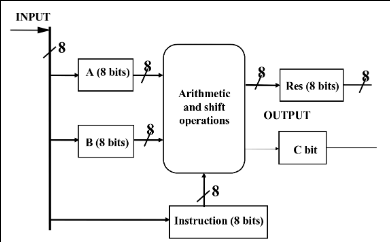
\includegraphics[]{2019-04-08-15-00-51.png}
                PANOPTO 1:21:56
                \medskip

                \begin{figure}[h!]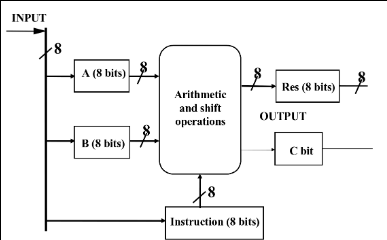
\includegraphics[width=\linewidth]{2019-04-08-20-08-22.png}\end{figure}

                For an $n$-bit ALU, there are $n + 1$ multiplexers, as the last one handles the carry bit. The $C_\text{in}$ bit for the $n^\text{th}$ multiplexer is the $C_\text{out}$ for the $(n - 1)^\text{th}$ multiplexer. The $C_\text{in}$ for the first multiplexer is 0.

\end{document}
